\documentclass[oneside]{article}


\usepackage{textcomp}
%change font. (ALTERNATIVE:  mathpazo, mathptmx, helvet, avant, courier, chancery, bookman, newcent, charter)
\usepackage{newcent} % math & rm 
\normalfont
\renewcommand{\ttdefault}{lmtt} %tt


\usepackage[english]{babel}
\usepackage[T1]{fontenc} % Use 8-bit encoding that has 256 glyphs
%\usepackage[latin3]{inputenc}
%\linespread{1.05} % Line spacing - Palatino needs more space between lines
\usepackage{microtype} % Slightly tweak font spacing for aesthetics
\usepackage[hmarginratio=1:1,top=32mm,columnsep=20pt]{geometry} % Document margins
\usepackage{multicol} % Used for the two-column layout of the document
\usepackage[hang, small,labelfont=bf,up,textfont=it,up]{caption} % Custom captions under/above floats in tables or figures
\usepackage{booktabs} % Horizontal rules in tables
\usepackage{float} % Required for tables and figures in the multi-column environment - they need to be placed in specific locations with the [H] (e.g. \begin{table}[H])
\usepackage{hyperref} % For hyperlinks in the PDF
\usepackage{lettrine} % The lettrine is the first enlarged letter at the beginning of the text
\usepackage{paralist} % Used for the compactitem environment which makes bullet points with less space between them
\usepackage{lipsum} % Package to generate dummy text throughout this template
\usepackage{graphicx}
%abstract
\usepackage{abstract} % Allows abstract customization
\renewcommand{\abstractnamefont}{\normalfont\bfseries} 
\renewcommand{\abstracttextfont}{\normalfont\small} 

%titolo
\usepackage{titlesec} 
\renewcommand\thesection{\Roman{section}}
\renewcommand\thesubsection{\Roman{subsection}} 
\titleformat{\section}[block]{\Large\bfseries\scshape\centering}{\thesection.}{1em}{} 
\titleformat{\subsection}[block]{\large\scshape}{\thesubsection.}{1em}{} 
\titleformat{\subsubsection}[block]{\scshape}{\thesubsubsection.}{1em}{} 




%headers & footers 
\usepackage{fancyhdr} % Headers and footers
\pagestyle{fancy} % All pages have headers and footers
\fancyhead[L]{\bfseries{{\textsf{Author}}}}
\fancyhead[R]{\bfseries{{\textsf{$\bullet$ Maradona $\bullet$ }}}}
%\fancyhead[R]{\small \leftmark}
\cfoot{\thepage}




%----------------------------------------------------------------------------------------
%	TITLE SECTION
%----------------------------------------------------------------------------------------
\thispagestyle{empty}


\title{\vspace{-15mm}\fontsize{24pt}{10pt}\selectfont\textsf{\bfseries{\textsc{D10s}}}} % Article title

\author{
\large
\textsc{Author}\\
\small \href{mailto:enter_adress_here}{\texttt{adress[dot]com}} 
%\vspace{-5mm}
}

\date{}

%----------------------------------------------------------------------------------------




\begin{document}

\maketitle % Insert title
\tableofcontents
\thispagestyle{empty} 

%----------------------------------------------------------------------------------------
%	ABSTRACT
%----------------------------------------------------------------------------------------

\begin{abstract}



\noindent Diego Armando Maradona is an Argentine football manager and retired professional footballer. He is widely regarded as one of the greatest football players of all time. 

\vspace*{4mm}
\end{abstract}




%----------------------------------------------------------------------------------------
%	ARTICLE CONTENTS
%----------------------------------------------------------------------------------------

\begin{multicols*}{2} % Two-column layout throughout the main article text



%-----------------------------------------------------1= INTRODUZIONE
\section{Foreword}

\lettrine{M}{aradona's} vision, passing, ball control and dribbling skills were combined with his small stature (1.65 m or 5 ft 5 in), which gave him a low center of gravity allowing him to maneuver better than most other football players; he would often dribble past multiple opposing players on a run. His presence and leadership on the field had a great effect on his team's general performance, while he would often be singled out by the opposition. A precocious talent, Maradona was given the nickname \emph{El Pibe de Oro} (The Golden Boy), a name that stuck with him throughout his career.





%----------------------------------------------------2= 

\section{Section A}

%\subsection{Soggetto}
\lettrine{D}{iego} Armando Maradona was born on 30 October 1960, at the Policlinico (Polyclinic) Evita Hospital in Lanus, Buenos Aires Province, but raised in Villa Fiorito, a shantytown on the southern outskirts of Buenos Aires, Argentina, to a poor family that had moved from Corrientes Province. He was the first son after three daughters. He has two younger brothers, Hugo (el Turco) and Raul (Lalo), both of whom were also professional football players. His parents were Diego Maradona "Chitoro" (d. 2015) and Dalma Salvadora Franco 'Dona Tota' (1930-2011). They were both born and brought up in the town of Esquina in the north-east province of Corrientes Province, living only two hundred metres from each other on the banks of the Corriente River. In 1950, they left Esquina and settled in Buenos Aires. At age eight, Maradona was spotted by a talent scout while he was playing in his neighbourhood club Estrella Roja. He became a staple of Los Cebollitas (The Little Onions), the junior team of Buenos Aires's Argentinos Juniors. 

As a 12-year-old ball boy, he amused spectators by showing his wizardry with the ball during the halftime intermissions of first division games. He named Brazilian playmaker Rivelino and Manchester United winger George Best among his inspirations growing up.\footnote{Footnote with active \href{<https://www.rte.ie/sport/soccer/2005/1126/198627-bestg/>}{link}}

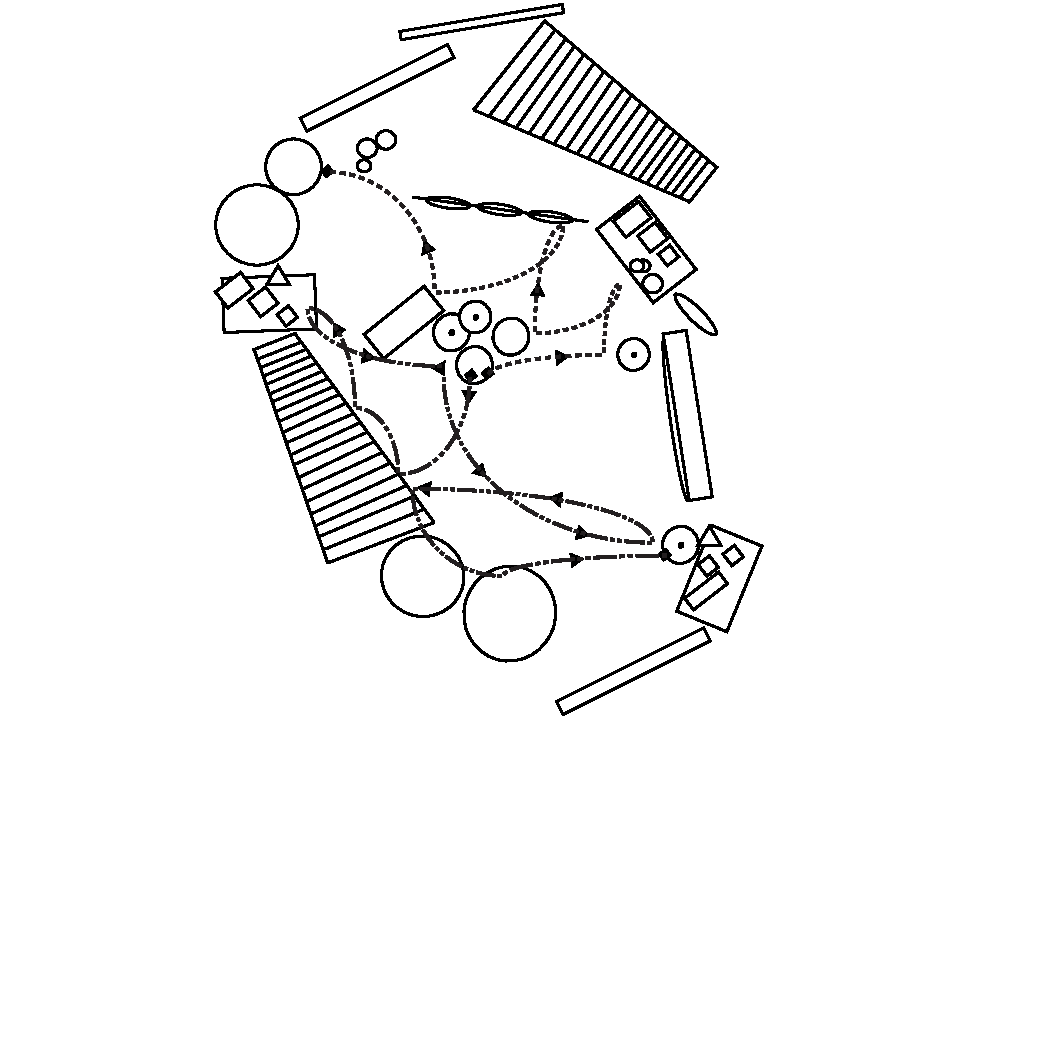
\includegraphics[width=0.4\textwidth]{img/percussions.pdf}


\section{Section B}

	
\lettrine{M}{aradona} arrived in Naples and was presented to the world media as a Napoli player on 5 July 1984, where he was welcomed by 75,000 fans at his presentation at the Stadio San Paolo.[43] Sports writer David Goldblatt commented, 
\begin{quote}
They (the fans) were convinced that the saviour had arrived.
\end{quote} 

A local newspaper stated that despite the lack of a \emph{mayor, houses, schools, buses, employment and sanitation, none of this matters because we have Maradona.} 

Prior to Maradona's arrival, Italian football was dominated by teams from the north and centre of the country, such as A.C. Milan, Juventus, Inter Milan and Roma, and no team in the south of the Italian Peninsula had ever won a league title.

\begin{center}
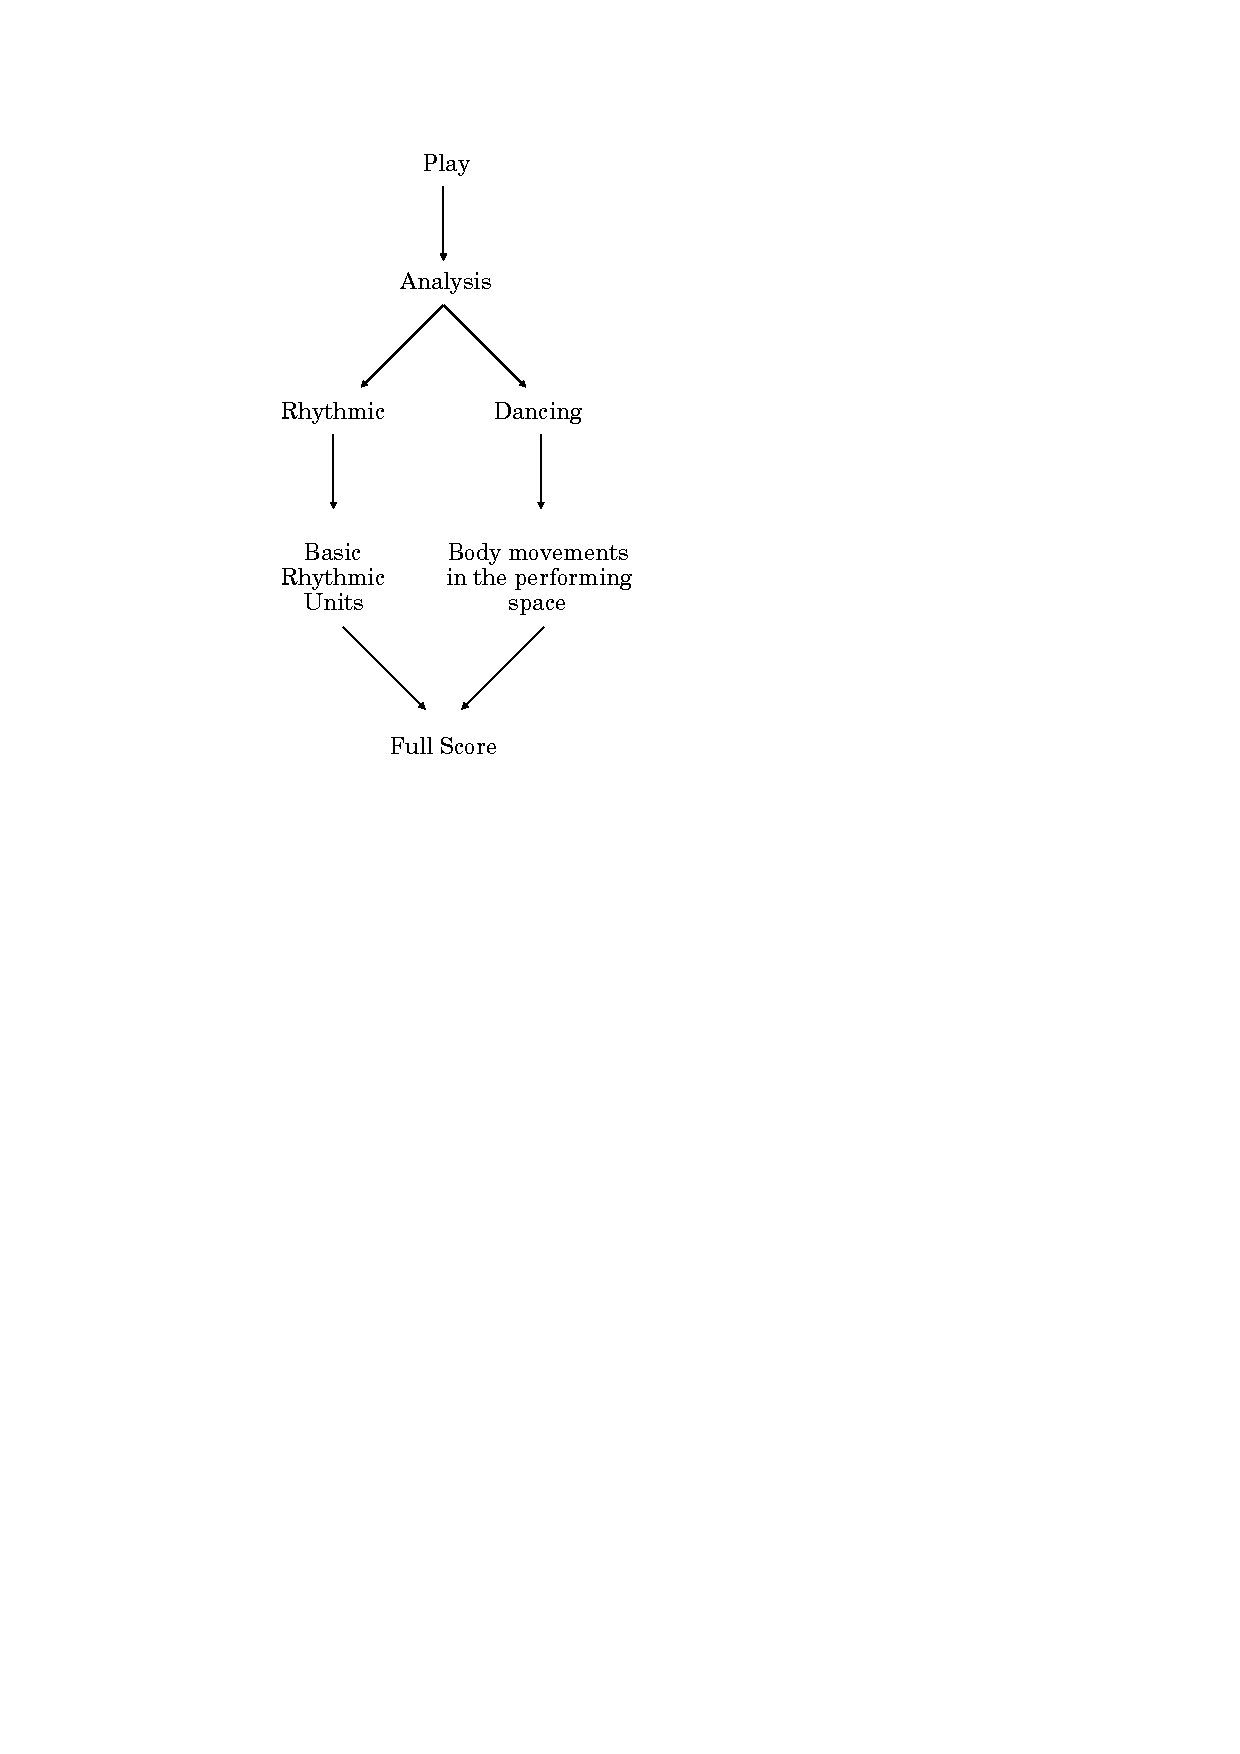
\includegraphics[width=0.3\textwidth]{img/schema.pdf}
 \end{center}
 
 
Napoli would win their second league title in 1989-90, and finish runners up in the league twice, in 1987-88 and 1988-89. Other honors during the Maradona era at Napoli included the Coppa Italia in 1987, (second place in the Coppa Italia in 1989), the UEFA Cup in 1989 and the Italian Supercup in 1990.Despite primarily playing in a creative role as an attacking midfielder, Maradona was the top scorer in Serie A in 1987-88, with 15 goals, and was the all-time leading goalscorer for Napoli, with 115 goals, until his record was broken by Marek Ham\v{s}ik in 2017.When asked who was the toughest player he ever faced, A.C. Milan central defender Franco Baresi stated, 
\begin{quote}
Maradona; when he was on form, there was almost no way of stopping him
\end {quote} 
a view shared by his Milan teammate Paolo Maldini, who stated, 
\begin{quote}
The best ever I played against was Maradona.
\end{quote}

\vspace{1cm}
%===============================================

\textbf{\textsf {Biblio}}\\
•\textsc{\textsf {Name Surname}}, \emph{Title}, Editor 1990\\
•\textsc{\textsf {Name Surname}}, \emph{Title}, Editor 2000\\





\end{multicols*}

\end{document}
